\documentclass[10pt]{article}
\usepackage{icmlko}

\icmlmeta{IP 파운데이션 월드모델}{288}{표지 하나가 모형을 이긴다}{노트 133이 채택한 넓힌 팝업 판이 이미 시장 레코드를 섞고 있었다 --- 마스크 무늬 하나가 모형보다 잘 맞힌다}

\begin{document}

\twocolumn[
\icmlheader

\begin{abstract}
노트 287이 ``넓힌 팝업 판이 더한 행에 파생 필드가 없다''를 남겼다. 왜인지
팠다. \textbf{그 114행 중 100행이 시장 레코드(\texttt{MKT-*})다.} 즉 넓힌
팝업 판은 \emph{이미} 내부와 시장을 섞어 놓은 판이고, \textbf{노트 283이
``붙이면 안 된다''고 한 구성 그대로}다. 재 봤다: 189행 중 시장 107, 손 축
다섯의 마스크가 \textbf{내부 98.8\% 대 시장 0.0\%}, 라벨은 시장이 2.05배,
그리고 \textbf{유보에서 관측 표시자 하나로 $|\rho|{=}0.4157$} 이다 ---
\textbf{같은 판의 실제 팝업 점수 0.3582 보다 크다.} \texttt{forms.\_design}
이 축마다 (값, 관측 표시자) 쌍을 내므로 그 표지는 명시적 열이고, 모형은
축을 안 보고 ``손 축이 있나'' 하나로 순위를 맞출 수 있다. \textbf{다만
정보가 있는 결측과 구별해야 한다} --- 게임의 \texttt{media\_push} 도 표시자가
라벨과 $+$0.405 인데 그건 ``자료가 있느냐''가 크기를 말하는 것이고 예측
시점에 아는 정보다. 가르는 표지를 찾았다: \textbf{뭉치가 축 계열을
가로지르나.} 넓힌 팝업은 한 뭉치 여덟이 공유 축과 검색을 함께 묶고, 게임은
검색끼리 · 위키끼리 따로 묶인다. \textbf{한 자료원 안의 동시 결측은
정상이고 계열을 가로지르는 동시 결측은 행의 출처가 다르다는 뜻이다.}
가드 열아홉 \textbf{출처}로 넣었다. 판정: 챔피언 판 \textbf{통과}(오염 없음) ·
\texttt{wide*} 둘 \textbf{실패} · 그리고 노트 284의 \texttt{trendcalwikitagmkt}
\textbf{통과} --- \textbf{시장을 붙이지 않고 따로 연 결정이 통과의 이유다.}
\end{abstract}
]

\section{넓힌 판이 이미 섞여 있었다}

노트 287이 넓힌 팝업 판에서 \texttt{pop\_*} 마스크가 43\% 로 떨어지는 것을
보고 ``넓힌 판이 더한 행에 파생 필드가 없다''로 끝냈다. 왜 없는지 팠다.

\begin{center}\small
\begin{tabular}{lr}
\hline
넓힌 판이 더한 행 & 114 \\
그중 \texttt{data/records/} 에 파일 있는 것 & \textbf{14} \\
없는 100개의 접두사 & \textbf{전부 \texttt{MKT}} \\
\hline
\end{tabular}
\end{center}

\textbf{시장 레코드다.} 넓힌 팝업 판 189행은 내부 82 $+$ 시장 107 이다.
노트 133이 이 판을 채택한 것이 노트 127$\sim$133 무렵이고, 그때는 시장 층이
없었으니 이후 병합에서 흘러든 것이다.

\section{표지 하나가 모형을 이긴다}

\begin{figure*}[t]
\centering
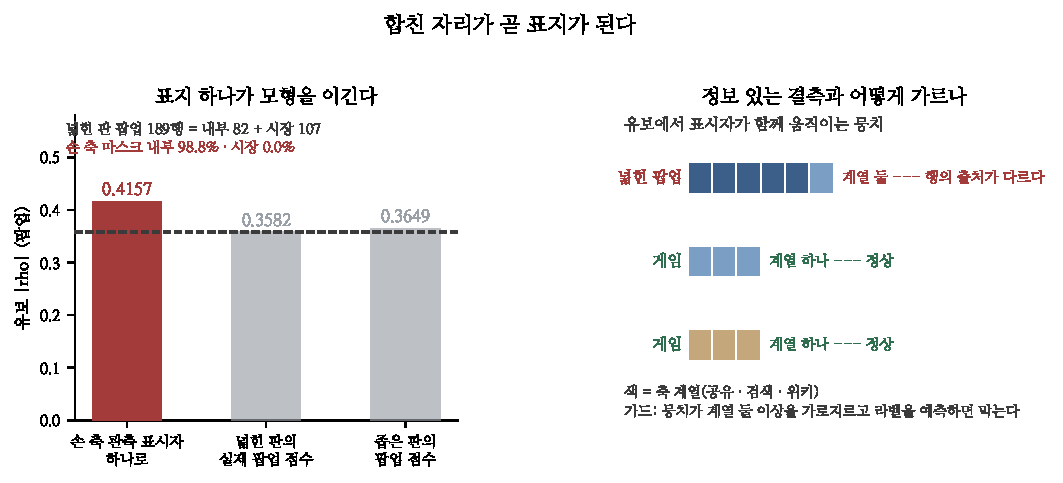
\includegraphics[width=\textwidth]{figs/marker.pdf}
\caption{왼쪽 --- 넓힌 팝업 판에서 관측 표시자 하나의 유보 $|\rho|$ 와 실제
점수. 오른쪽 --- 표시자가 함께 움직이는 뭉치가 축 계열을 가로지르나.}
\end{figure*}

\begin{center}\small
\begin{tabular}{lrr}
\hline
& 내부 82 & 시장 107 \\
\hline
손 축 다섯 마스크 & \textbf{98.8\%} & \textbf{0.0\%} \\
라벨 중앙(log10 일평균) & 2.773 & 3.084 \\
\hline
\multicolumn{3}{l}{차 $+$0.311 $=$ \textbf{2.05배}} \\
\hline
\end{tabular}
\end{center}

\begin{center}\small
\begin{tabular}{lr}
\hline
유보에서 & $|\rho|$ \\
\hline
\textbf{손 축 관측 표시자 하나} & \textbf{0.4157} \\
넓힌 판의 실제 팝업 점수 & 0.3582 \\
(참고) 좁은 판의 팝업 점수 & 0.3649 \\
\hline
\end{tabular}
\end{center}

\textbf{표지가 모형보다 잘 맞힌다.} 표시자와 출처가 99.5\% 일치하므로 사실상
``이 행이 어느 자료집에서 왔나''를 읽는 것이다. \texttt{forms.\_design} 이
축마다 \textbf{(값, 관측 표시자)} 쌍을 내니 그 열은 모든 정식화에 그냥
주어져 있다.

\paragraph{노트 127 · 133의 근거를 다시 봐야 한다} 그 노트들은 넓힌 판의
팝업 이득($+$0.3688 $\to$ $+$0.4495)을 ``팝업이 학습 풀에 들어가서''로
설명했다. \textbf{출처 표지도 같은 모양의 이득을 낸다} --- 어느 쪽인지 그때
안 갈랐다. 지금 판에서 표지 하나가 0.4157 이니 \textbf{가능성이 아니라
크기가 맞는 대안 설명}이다.

\section{정보 있는 결측과 어떻게 가르나}

여기서 조심할 것이 있다. \textbf{표시자가 라벨을 예측한다고 다 병이 아니다.}

\begin{center}\small
\begin{tabular}{lrl}
\hline
& 표시자 $\rho$ & \\
\hline
게임 \texttt{media\_push} & $+$0.405 & \textbf{정당하다} \\
게임 \texttt{wiki\_level} & $+$0.397 & \textbf{정당하다} \\
넓힌 팝업 손 축 & $-$0.416 & 병 \\
\hline
\end{tabular}
\end{center}

게임 쪽은 ``자료가 있느냐''가 실제로 크기를 말하는 것이다 --- 미디어 자료가
안 잡히는 게임은 작다. 그리고 \textbf{예측 시점에 아는 정보}라 써도 된다.
넓힌 팝업 쪽은 ``어느 파일에서 읽어 왔나''라서 세상의 성질이 아니다.

\paragraph{가르는 표지} 상관만으로는 못 가른다. 무늬를 봤다.

\begin{center}\small
\begin{tabular}{lll}
\hline
& 함께 움직이는 뭉치 & 계열 \\
\hline
넓힌 팝업 & 축 \textbf{여덟}이 한 뭉치 & 공유 $+$ 검색 \textbf{(둘)} \\
게임 & 검색끼리 셋 & 검색 (하나) \\
게임 & 위키끼리 셋 & 위키 (하나) \\
\hline
\end{tabular}
\end{center}

\textbf{한 자료원 안의 동시 결측은 정상이다} --- 검색을 못 긁으면 검색 축
셋이 같이 빈다. \textbf{계열을 가로지르는 동시 결측은 행의 출처가 다르다는
뜻이다} --- 손으로 태깅한 축과 크롤링한 검색 축이 \emph{같이} 빌 이유는
그 행이 다른 파일에서 왔을 때뿐이다.

\section{가드 열아홉 --- 출처}

유보에서 표시자가 $|\rho|{\ge}0.95$ 로 함께 움직이는 뭉치(셋 이상)를 찾고,
그 뭉치가 \textbf{축 계열 둘 이상}을 가로지르면서 라벨을 $|\rho|{\ge}0.25$ 로
예측하면 막는다. 라벨을 보므로 \textbf{거부권으로만} 쓴다(노트 183).

\begin{center}\small
\begin{tabular}{ll}
\hline
축 세트 & 판정 \\
\hline
\texttt{trendcalwikitag}(챔피언) & \textbf{통과} --- 오염 없음 \\
\texttt{wide\_trendcal} & 실패 (축 8 · 계열 둘 · $\rho{=}{-}0.387$) \\
\texttt{wide\_trendcalpop} & 실패 (축 12 · 계열 셋) \\
\textbf{\texttt{trendcalwikitagmkt}} & \textbf{통과} \\
\hline
\end{tabular}
\end{center}

마지막 줄이 이 노트에서 제일 반가운 것이다. \textbf{노트 283 · 284가 시장
층을 팝업에 \emph{붙이지 않고} 열한 번째 도메인으로 연 결정}, 그것이 통과의
이유다 --- 도메인 안에서 마스크 무늬가 균일하면 표지가 안 생긴다. \textbf{그때
손으로 내린 판단을 이제 가드가 자동으로 한다.}

\paragraph{한철과 정반대다} 가드 \textbf{한철}(노트 214)은 지표가 \emph{유보에서
상수}일 때를 잡는다(학습만 가르는 스위치). 이것은 지표가 유보에서 \emph{변하면서
라벨을 예측할} 때를 잡는다. \textbf{같은 열의 두 반대 무늬에 가드가 하나씩
붙었다.}

\paragraph{덤 --- 분모 가드도 같이 걸었다} 시장팝업을 열자 가드 \textbf{분모}가
``추가 [시장팝업] (기준 9개)''로 걸렸다. 설계대로다(노트 82 · 90). 의도한
변경이라 \texttt{denominator.json} 기준을 9 $\to$ 10 으로 \emph{명시적으로}
다시 놓고 이유를 적었다. \textbf{지문 · 분모 · 출처 셋이 같은 사건을 각각
잡았다.}

\paragraph{남은 것}
\begin{center}\small
\begin{tabular}{ll}
\hline
갈래 & 왜 \\
\hline
넓힌 판을 어떻게 할까 & 시장 107행을 떼거나 도메인을 가르거나 \\
노트 127 · 133 재검토 & 그 이득이 표지였나 학습 풀이었나 \\
좁은 판의 MKT 7건 & 유보 5건이 15.4배 --- 라벨 잡음 \\
가드를 옛 판에 & \texttt{wide*} 를 쓴 노트들 표시 \\
\hline
\end{tabular}
\end{center}

\paragraph{규약} \textbf{두 자료를 한 도메인에 넣으면 결측 무늬가 출처를
말하고, 출처가 라벨을 말한다.} 노트 283이 손으로 내린 이 판단을 가드로
옮겼다. 그리고 \textbf{``표시자가 라벨을 예측한다''만으로는 병인지 신호인지
못 가른다} --- 뭉치가 계열을 가로지르는지 봐야 한다.

\end{document}
